%!TEX root = ../thesis_main.tex

%%%%%%%%%%
\chapter{Software Requirements Specification and Structured Analysis}
\label{chap:srs-sa}
%%%%%%%%%%

This chapter deals with the Software Requirement Specification (SRS) \cite{IEEE8301998} and the Structured Analysis \cite{SA_Braune} of the system developed in this work. Thanks to these two procedures, the objectives that the system must fulfil and a decomposition of it into different functions are stated. This leads to a complete definition of the system.

\nomenclature[ba]{SRS}{Software Requirement Specification}

The purpose of this work is to design a Visual Servoing controller to provide an underactuated aerial robot the commands necessary to reach a desired pose with respect to a target object.

The VS controller developed is to be integrated into the hector\_quadrotor \cite{2012simpar_meyer}, an underactuated aerial robot equipped with a monocular monochrome camera pointing downwards.

%%%%%%%%%%
\section{Software Requiremet Specification}
\label{sec:srs}
%%%%%%%%%%

In this section the Software Requirement Specification \cite{IEEE8301998} for the Visual Servoing controller developed in this thesis is presented. Using SRS helps to define the system that is being designed, tracking continuously that the product developed satisfies the needs of the user. Only when every requirement stated therein is fulfilled the implementation would be completed.

%%%%%%%%%%
\subsection{Product Perspective}
\label{sec:product-perspective}
%%%%%%%%%%

The VS controller is to be used with an aerial robotic system based on the ROS framework. From the perspective of the robotic system, the VS controller subsystem will appear as a ROS node which publishes control commands through a ROS topic to the rest of the system.

The used aerial robotic system is the hector\_quadrotor\footnote{\url{wiki.ros.org/hector_quadrotor}} model \cite{2012simpar_meyer}. (TODO: Add diagram).

The subsystem developed here is to interact with the camera hardware of the robot, a monocular monochrome camera pointing downwards (TODO: Add hardware). The output of the subsystem are the control inputs of the aerial robot dynamics (TODO: Add which are the quadrotor control inputs), this inputs interact with the inner control loop for the attitude and outer control loop for the position already implemented in the robotic system (TODO: Position loop is not related to vs system, but can be useful for benchmark).

%%%%%%%%%%
\subsection{User Characteristics}
\label{sec:user-characteristics}
%%%%%%%%%%

The product developed in this thesis will be used as part of a ROS-based system, thus the expected user is a designer willing to implement a VS control strategy for his robotic system. The user should be familiarized with the ROS framework and the system will need the structure and interfaces of any standard ROS product.

%%%%%%%%%%
\subsection{Assumptions and Dependencies}
\label{sec:assumptions-dependencies}
%%%%%%%%%%

The software  has been tested on the following platforms, forward or backward support is not guaranteed on a different set-up.

\begin{itemize}
	\item ROS version: ROS Indigo\footnote{\url{http://wiki.ros.org/indigo}}
	\item Operating System: Ubuntu 14.04\footnote{\url{http://releases.ubuntu.com/14.04/}} Trusty Tahr, 64 bit
\end{itemize}

%%%%%%%%%%
\subsection{Functional Requirements}
\label{sec:functional-requirements}
%%%%%%%%%%

The functional requirements describe what the system must do to complete the overall task:

\begin{itemize}
	\item F1: \emph{Give visual servoing control input}. Control input based on image data so that the aerial robot comes closer to the target pose. Control as a difference on the image features, no pose estimation.
	\item F2: \emph{Tell user when the target pose is achieved}. The system must be able of telling the user whether the target pose has been already achieved or not.
\end{itemize}

%%%%%%%%%%
\subsection{Other Requirements}
\label{sec:other-requirements}
%%%%%%%%%%

\begin{itemize}
	\item A1: All components are working reliably.
	\item A2: The software is sufficiently fast, modular and modifiable.
	\item A3: The implementation is transparent and comprehensible.
	\item A4: Control inputs must provide stable and smooth flight manoeuvres.
	\item A5: Robot must be able to start from different initial positions.
	\item A6: Algorithm must be fast enough to allow real time control of the aerial robot.
	\item A7: The implementation should follow the style guide of ROS\cite{ROS_Style}
\end{itemize}

%%%%%%%%%%
\subsection{General Constraints}
\label{sec:general-constraints}
%%%%%%%%%%

\begin{itemize}
	\item The environment must be sufficiently illuminated for the camera to work.
	\item The target pose must be provided by a sufficient number of features (TODO: How many?) in form of a 2D code (TODO: At least in the first
version).
	\item The target must be always in the filed of view of the camera, so features can be extracted an control input computed.
	\item Testing computer is a MacBook Pro\footnote{\url{https://everymac.com/systems/apple/macbook_pro/specs/macbook-pro-core-i5-2.7-13-early-2015-retina-display-specs.html}} (Early 2015) with 2.7 GHz Intel Core i5 processor, 8 GB 1867 MHz DDR3 memory and Intel Iris Graphics 6100 1536 MB graphics. Linux OS is run using Oracle VM VirtualBox\footnote{\url{www.virtualbox.org}} (Version 5.1.14 r112924) with 5 GB base memory and two processors.
\end{itemize}

\nomenclature[ba]{OS}{Operative System}

%%%%%%%%%%
\section{Structured Analysis}
\label{sec:sa}
%%%%%%%%%%

\begin{figure}[h]
	\centering
	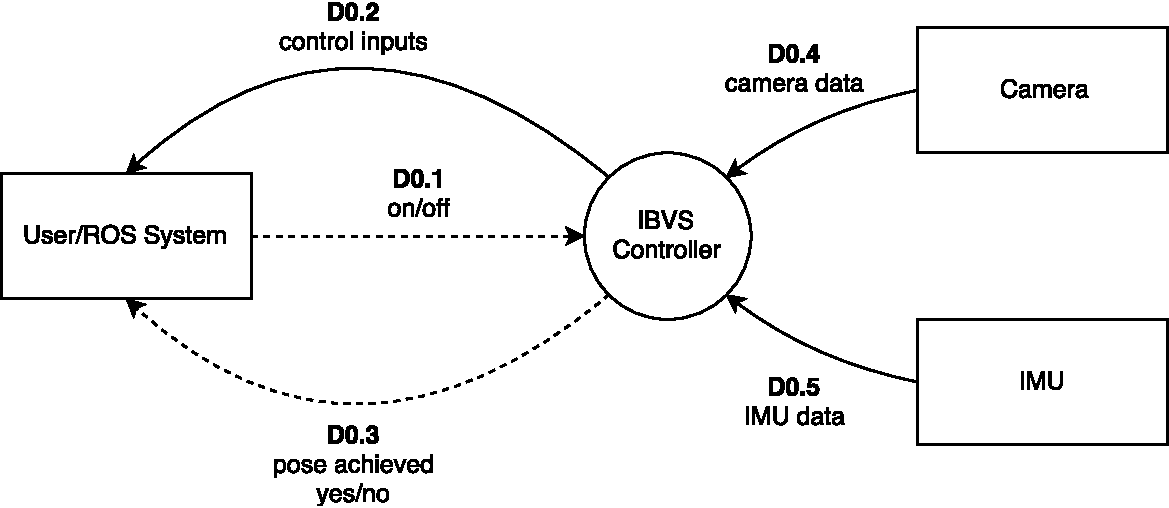
\includegraphics[width=\textwidth]{content/chapter_03/images/sa_diagram_01_01.pdf}
	\caption{Context diagram}
	\label{fig:sa_diag_01}
\end{figure}

